
\begin{figure*}[!t]
  \centering
  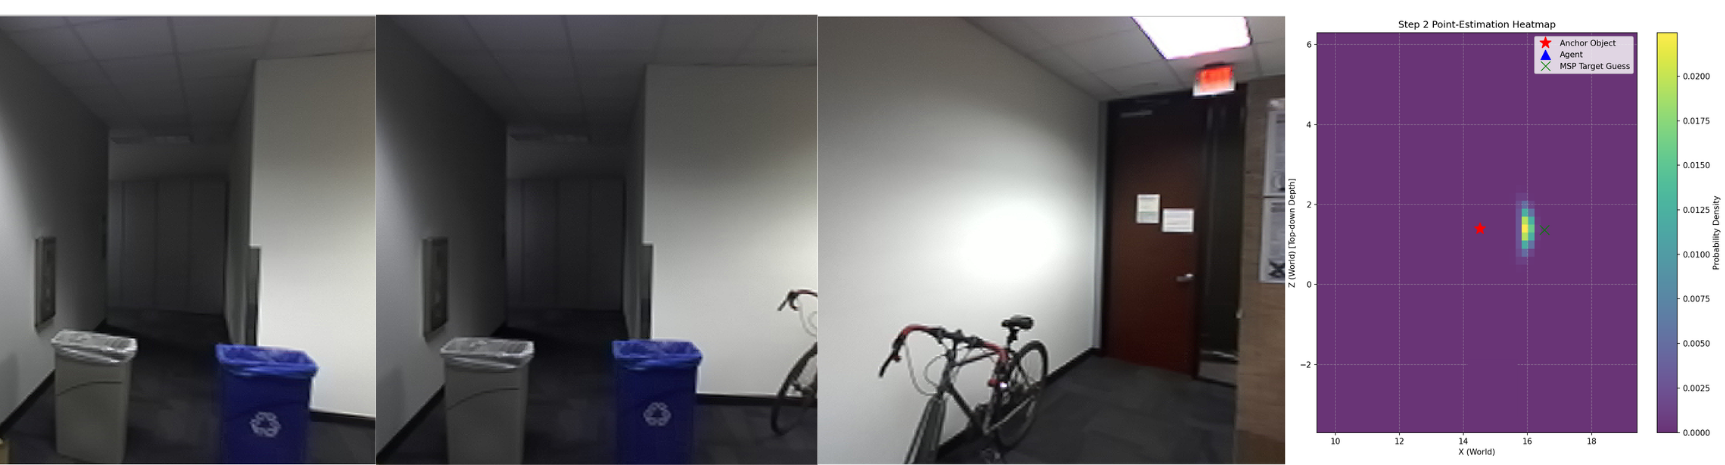
\includegraphics[width=\textwidth]{figures/fig_6_robot.png}
  \caption{\rev{\textbf{Real-world MAPG grounding example.} Using observations collected from a Robotis AI Worker robot, we construct an offline scene graph of a physical indoor environment. Three egocentric image frames are shown, with the query ``Where is $1$ meter to the right of the trash can close to the bicycle?'' MAPG infers a spatial probability distribution over candidate goal locations (right). The anchor (red) and predicted goal (green) illustrate metrically consistent semantic grounding in a physical environment: the grounded area is $1\,\mathrm{m}$ to the right of the blue trash can, consistent with the bicycle's position.}}
  \label{fig:obs-anchor-trace}
\end{figure*}

\section{Observations and Discussions}
\label{sec:observations}
% \opnote{IMP: need more numbers everywhere, even in the text. ...}
%\opnote{Lots of redundant stuff in this section. You should make it denser.}

The completed Claude Opus 4.6 run succeeded on $79$ of $98$ episodes ($80.6\%$) and found the anchor on $80$ ($81.6\%$). Tables~\ref{tab:predicate_success} and~\ref{tab:distance_success} provide the corresponding breakdowns, with the small-cell caution stated alongside them.
Tables~\ref{tab:mapg_bench}--\ref{tab:ablations_occlusion} show that MAPG's gains stem from two design choices:
% \opnote{bad language, say improvements are shown through results and point to tables.}
\textbf{(i) query decomposition} (anchor / predicate / metric) and \textbf{(ii) probabilistic composition} of per-clause kernels into a planner-queryable goal density. On MAPG-Bench, MAPG (GPT-5.2) reduces O-W error from $5.82\,\mathrm{m}$ to $0.07\,\mathrm{m}$ and improves TSR from $0.78$ to $0.98$. Ablations in Tables~\ref{tab:ablations_spatial} and~\ref{tab:ablations_occlusion} show %\opnote{bad language. Ablations in Table XYZ show that ...}
that these gains are primarily due to our compositional framework 
% \opnote{primarily due to our compositional framework}
rather than ``better prompting'': removing the spatial reasoner drops object-selection SR from $0.42$ to $0.20$, and under occlusion, explicit reasoning recovers SR from $0.30$ to $0.50$.

\noindent\textbf{Multi-view evidence accumulation enables reliable anchor disambiguation.}
The Grounding Agent iterates over egocentric views, accumulates CLIP-scored evidence, and maintains a blacklist of Verifier-rejected candidates, deferring commitment until confidence exceeds threshold. This behavior directly explains MAPG's high Anchor Pick SR (up to $0.98$, vs.\ GraphEQA's $0.48$). GraphEQA selects the nearest scene-graph match at the first step; under partial observability this commits to the wrong instance roughly half the time. The occlusion ablation confirms this: when the anchor is initially occluded, MAPG's iterative belief update recovers upon re-observation, whereas CoT-only reasoning has no mechanism to revise its initial commitment.

\noindent\textbf{Log-space kernel composition yields planner-ready allocentric waypoints.}
MAPG's final waypoint is the peak of a composed density over $\Omega_{\text{free}}$: $\log P(x) = \ell_{\text{met}} + \ell_{\text{dir}}$ for O-W goals, with the semantic kernel acting on anchor selection rather than goal placement (Eqs.~\ref{eq:shrinkage}--\ref{eq:ow-composition}). Crucially, this is an \emph{allocentric} $3$D coordinate directly consumable by RRT*~\cite{karaman2011sampling}, with no interpretation step required. GraphEQA's large O-W error ($5.82\,\mathrm{m}$) and yaw error ($13.50^\circ$) arise because its nearest-satisfying heuristic enforces direction but ignores the metric offset; MAPG's metric kernel explicitly penalizes deviation from $d_0$, collapsing the error to $0.07\,\mathrm{m}$ and $1.90^\circ$. MAPG's equivalent results on HM-EQA ($0.71$ TSR vs.\ $0.67$ for GraphEQA) confirm that the decomposition does not hurt when metric constraints are absent, while MAPG-Bench results confirm the full benefit emerges precisely when metric constraints and multi-predicate conjunctions stack together. 
% \opnote{sounds like chatgpt language. be more direct...}

\noindent\textbf{Failure modes and limitations.}
Most failures stem from limitations in the underlying scene representation. \emph{Scene-graph incompleteness} (occluded objects that never enter the map) forces grounding relative to a partial world model. \emph{Frame-of-reference ambiguity} is the dominant failure on the commonsense subset: for ``in front of the sofa,'' MAPG (Gemini 2.5 Pro) predicts the camera-centric front rather than the sofa's affordance-defined facing direction, placing the waypoint behind the sofa, precisely the VLM bias documented in~\cite{frameOfReferenceAmbiguity}. MAPG (Claude Opus 4.6) handles this better ($0.30$ vs.\ $0.14$ for GraphEQA) because the Orchestrator's \texttt{intrinsic\_front} label triggers object-frame kernel computation, but performance still falls short of perfect, reflecting limits in inferring affordance direction from partial views. Finally, misalignment between the free-space grid and the scene-graph coordinate frame can smear the composed belief map, reducing waypoint precision for anchors near walls or furniture.
% \opnote{as shown in XYZ} \opnote{IMP: need to add a failure example.}
